\documentclass[runningheads]{llncs}
%
\usepackage[T1]{fontenc}

\usepackage{graphicx}

% Package to create a symbols
\usepackage{amsmath}
\usepackage{amssymb}
\usepackage{amsfonts}

% Package to use the htbp option 
\usepackage{float} 
\usepackage{placeins}

\usepackage{colortbl}  % Required for \rowcolor
\usepackage{xcolor}    % Provides additional color definitions

% Package to insert code
\usepackage{listings}
\definecolor{comment}{RGB}{0,128,0}
\definecolor{string}{RGB}{255,0,0}
\definecolor{keyword}{RGB}{0,0,255}
\definecolor{lightgray}{rgb}{.9,.9,.9}
\definecolor{darkgray}{rgb}{.4,.4,.4}
\definecolor{purple}{rgb}{0.65, 0.12, 0.82}
\lstdefinestyle{codestyle}{
  commentstyle=\color{comment},
  stringstyle=\color{string},
  keywordstyle=\color{keyword},
  basicstyle=\footnotesize\ttfamily,
  numbers=left,
  numberstyle=\tiny,
  numbersep=5pt,
  frame=lines,
  breaklines=true,
  prebreak=\raisebox{0ex}[0ex][0ex]{\ensuremath{\hookleftarrow}},
  showstringspaces=false,
  upquote=true,
  tabsize=2,
}
\lstset{style=codestyle}

\lstdefinelanguage{JavaScript}{
  keywords={typeof, new, true, false, catch, function, return, null, catch, switch, var, if, in, while, do, else, case, break},
  keywordstyle=\color{blue}\bfseries,
  ndkeywords={class, export, boolean, throw, implements, import, this},
  ndkeywordstyle=\color{darkgray}\bfseries,
  identifierstyle=\color{black},
  sensitive=false,
  comment=[l]{//},
  morecomment=[s]{/*}{*/},
  commentstyle=\color{purple}\ttfamily,
  stringstyle=\color{red}\ttfamily,
  morestring=[b]',
  morestring=[b]"
}

% Package to use the \lipsum command
\usepackage{lipsum} 

% Package to use the \algorithm command
\usepackage{algorithm}
\usepackage{algpseudocode}


\begin{document}

%

\title{IRIS ITS Team Description}

% Insert your team name here
\author{Azzam Wildan \and
Second Author \and
Third Author \and 
Fourth Author}

% First names are abbreviated in the running head.
% If there are more than two authors, 'et al.' is used.
\authorrunning{Azzam, et al.}

% Insert your institute name, address, email, and website here
\institute{Institut Teknologi Sepuluh Nopember \\
ITS Campus, Sukolilo, Surabaya, Indonesia \\
\email{iris@krsbi.its.ac.id}\\
\url{https://www.its.ac.id}
}
%
\maketitle              
%
\begin{abstract}
    The abstract should briefly summarize the contents of the paper in
    150--250 words. \lipsum[20]
    
    \keywords{First keyword  \and Second keyword \and Another keyword.}
\end{abstract}
%
\section{Introduction}
IRIS-ITS is \lipsum[10]

\section{Mechanical Design}
\lipsum[11]

\section{Electrical Design}
\lipsum[30]

\section{Software Design}
\lipsum[30]

\subsection{Software Architecture}
\lipsum[30]





% It contains an example of using table and figure, 
% you can remove it if you don't need it
% Just add [H] after \begin{table} or \begin{figure} 
% It will place it exactly where you want it to be. 

\section{Example}

Example of using table 
\begin{table}[H]
    \caption{Table captions should be placed above the
    tables.}\label{tab1}
    \begin{tabular}{|l|l|l|}
    \hline
    Heading level &  Example & Font size and style\\
    \hline
    Title (centered) &  {\Large\bfseries Lecture Notes} & 14 point, bold\\
    1st-level heading &  {\large\bfseries 1 Introduction} & 12 point, bold\\
    2nd-level heading & {\bfseries 2.1 Printing Area} & 10 point, bold\\
    3rd-level heading & {\bfseries Run-in Heading in Bold.} Text follows & 10 point, bold\\
    4th-level heading & {\itshape Lowest Level Heading.} Text follows & 10 point, italic\\
    \hline
    \end{tabular}
\end{table} 


Example of using figure 
\begin{figure}[H]
    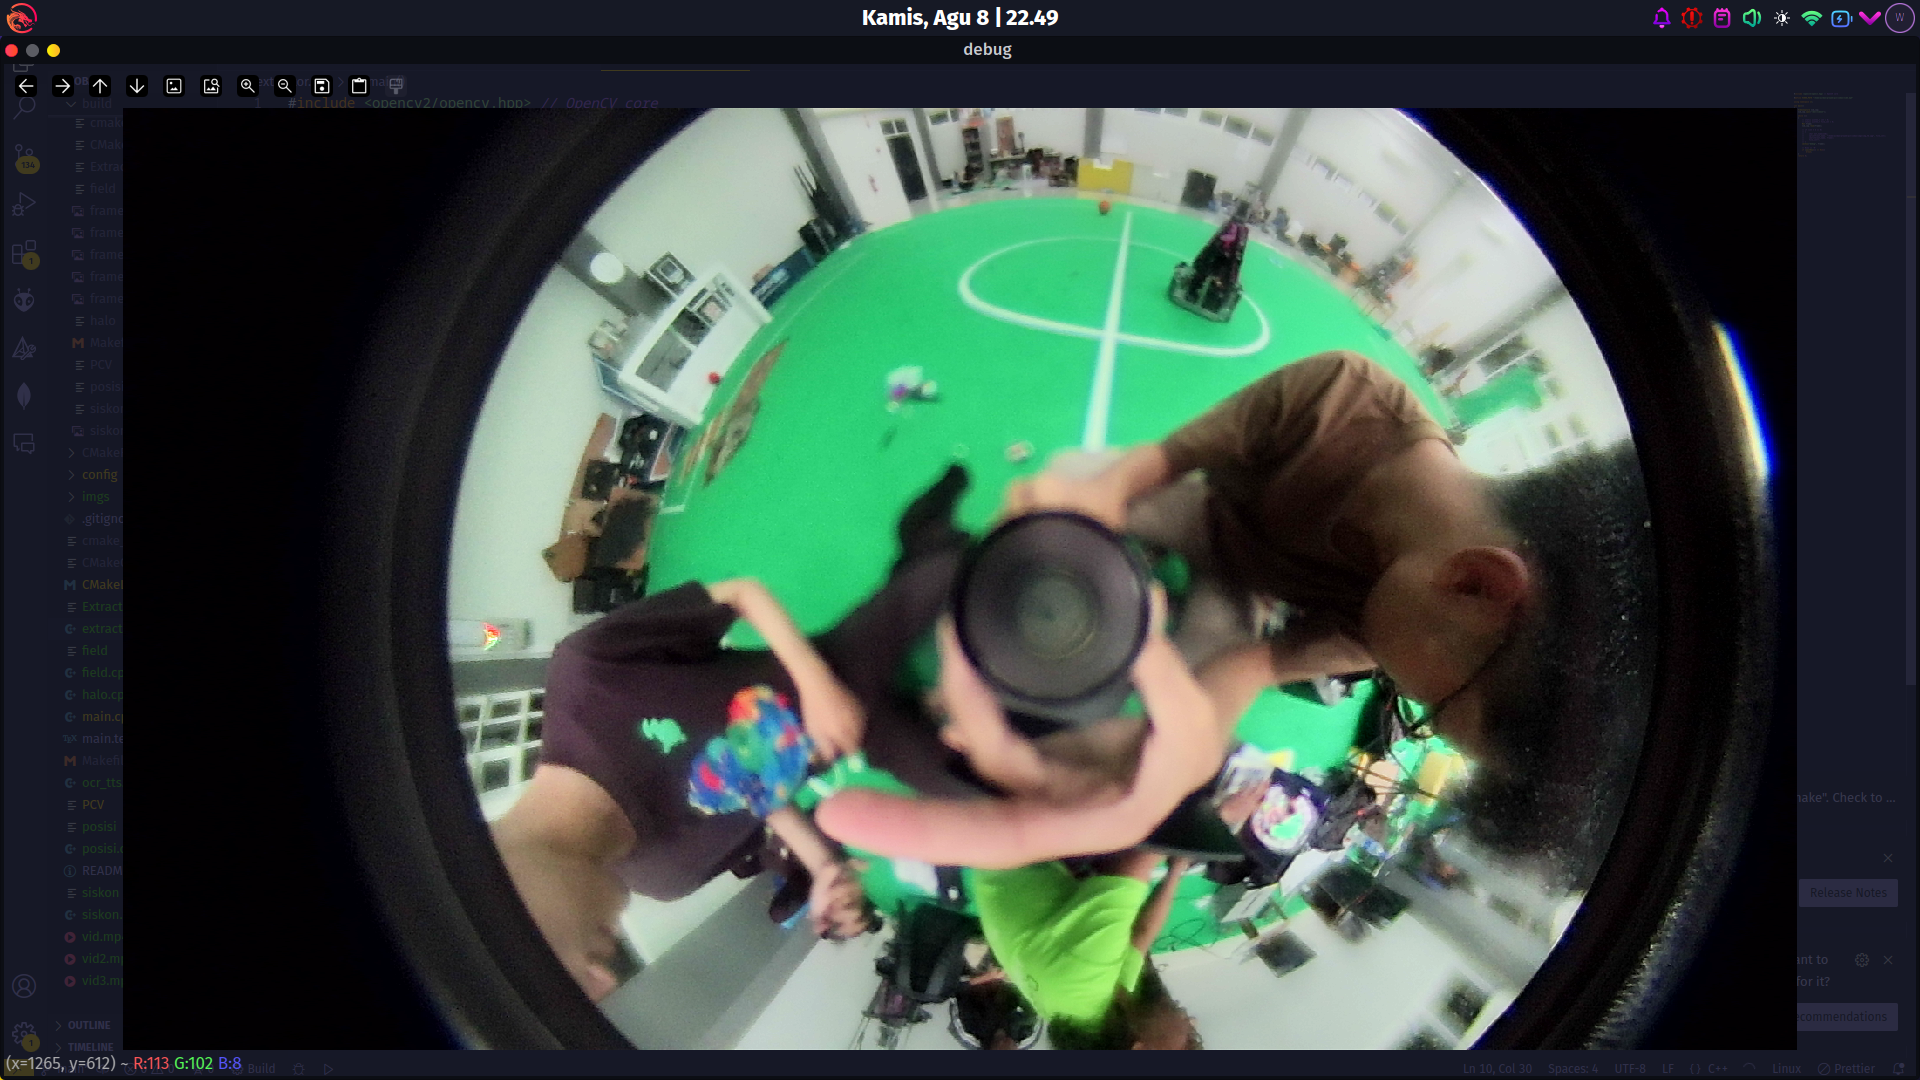
\includegraphics[width=\textwidth]{images/leopard3.png}
    \caption{A figure caption is always placed below the illustration.
    Please note that short captions are centered, while long ones are
    justified by the macro package automatically.} \label{fig1}
\end{figure}

Example of using equation 
\begin{equation}
    x + y = z
\end{equation}

Example of using theorem
\begin{theorem}
    Theorem content, for example: $x + y = z$
\end{theorem}

Example of using proof
\begin{proof}
    Proof content, for example: $x + y = z$
\end{proof}

Example of using algorithm
\begin{algorithm}[H]
    \caption{Process Lines on Frame}\label{alg:process_lines}
    \begin{algorithmic}[1]
    \Procedure{ProcessLinesOnFrame}{}
        \State \text{Initialize lines\_on\_frame as an empty vector}
        \For{\text{angle from 0 to 360 with step size 2.5}}
            \State \text{Initialize dist to 0}
            \For{\text{index from 0 to 320}}
                \State $x \gets \text{dist} \times \cos(\text{angle}) + \text{center\_cam\_x}$
                \State $y \gets \text{center\_cam\_y} - \text{dist} \times \sin(\text{angle})$
                \If{\text{frame[y][x] == 255}}
                    \State \text{Push (x, y) to lines\_on\_frame}
                \EndIf
                \State $dist \gets \text{dist} + 1$
            \EndFor
        \EndFor
    \EndProcedure
    \end{algorithmic}
\end{algorithm}

Example of using citation \cite{ref_url1}.



% If you want to add some references, you can use the following snippet:
\bibliographystyle{splncs04}
\bibliography{references}
\end{document}
